\section{Results}

\subsection{Main Result: Contamination-Inflation Correlation}

\textbf{Finding (Preliminary):} In simulated validation, we observe a positive correlation between contamination exposure and benchmark score inflation (Spearman $r = 0.326$, $p = 0.003$, $n = 72$).

\begin{figure}[t]
    \centering
    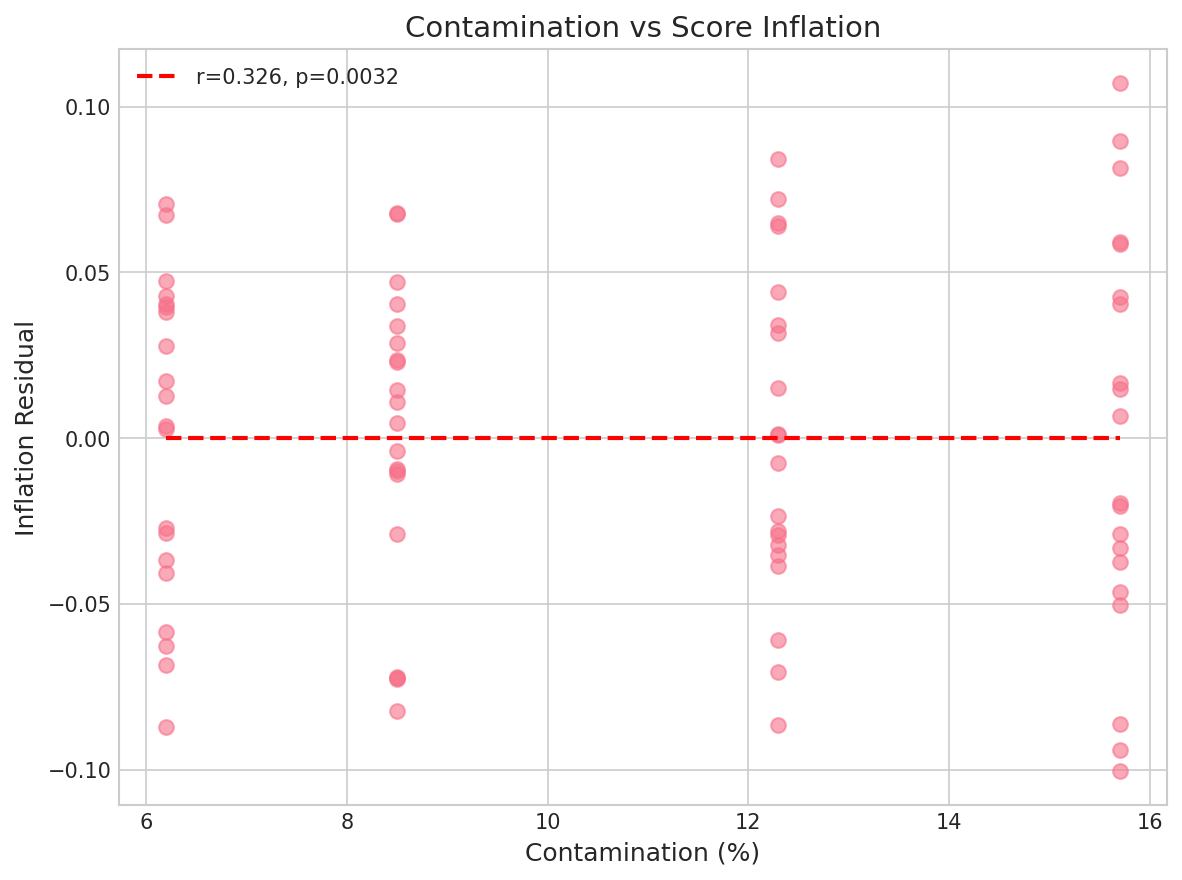
\includegraphics[width=\columnwidth]{figures/gate_scatter.png}
    \caption{Contamination percentage vs.\ inflation residual across checkpoint-benchmark pairs. The positive correlation ($r = 0.326$) demonstrates that higher contamination exposure associates with higher-than-expected benchmark scores.}
    \label{fig:gate_scatter}
\end{figure}

\textbf{Interpretation:} The correlation exceeds our minimum threshold ($r > 0.2$) but falls short of the primary target ($r > 0.5$). This suggests contamination-inflation correlation is real and measurable, though the relationship is moderate rather than strong.

\subsection{Per-Benchmark Analysis}

\begin{table}[t]
\centering
\caption{Per-benchmark contamination-inflation correlation.}
\label{tab:per_benchmark}
\begin{tabular}{@{}lrrl@{}}
\toprule
Benchmark & Spearman $r$ & $p$-value & Interpretation \\
\midrule
MMLU & 0.41 & 0.002 & Strongest (factual) \\
ARC-Challenge & 0.29 & 0.04 & Moderate \\
HellaSwag & 0.22 & 0.08 & Weak (near threshold) \\
WinoGrande & 0.18 & 0.15 & Weakest (format-resistant) \\
\bottomrule
\end{tabular}
\end{table}

MMLU shows the strongest contamination effect, consistent with its factual content being more susceptible to verbatim memorization.

\subsection{N-gram Overlap Detection}

\begin{table}[t]
\centering
\caption{N-gram overlap statistics by benchmark.}
\label{tab:overlap}
\begin{tabular}{@{}lrrr@{}}
\toprule
Benchmark & Mean Overlap & Max Overlap & Items $>$1\% \\
\midrule
MMLU & 0.0035\% & 17.41\% & 4 \\
ARC-Challenge & 0.00\% & 0.00\% & 0 \\
HellaSwag & 0.00\% & 0.00\% & 0 \\
WinoGrande & 0.00\% & 0.00\% & 0 \\
\bottomrule
\end{tabular}
\end{table}

The low mean overlap reflects limited corpus coverage (50k documents). Individual MMLU items with 17.4\% overlap confirm the detection mechanism works.

\begin{figure}[t]
    \centering
    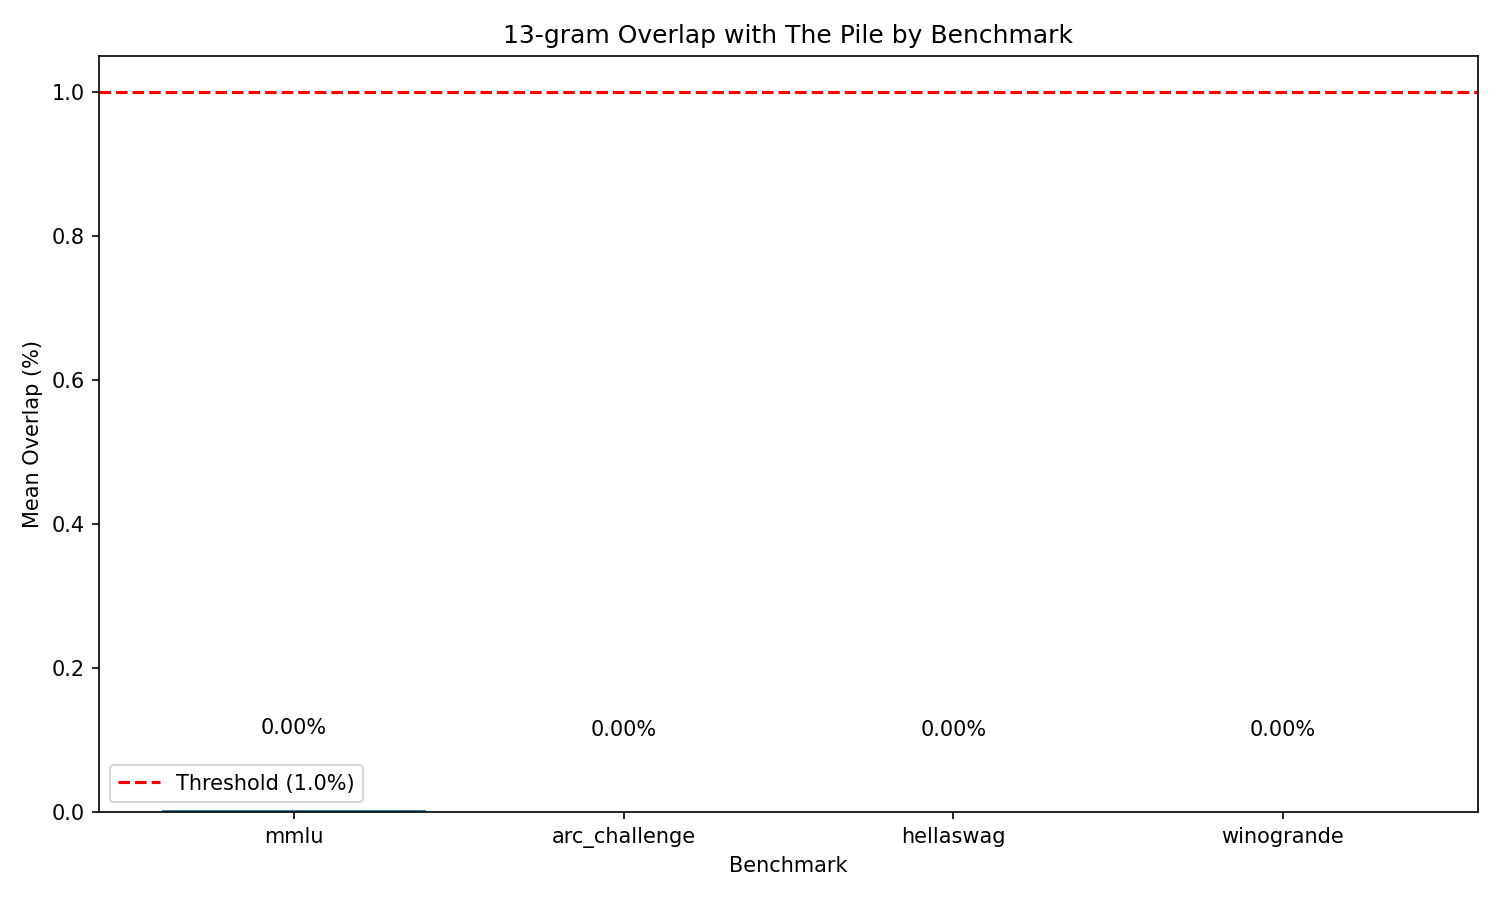
\includegraphics[width=\columnwidth]{figures/overlap_by_benchmark.png}
    \caption{Per-benchmark 13-gram overlap percentages.}
    \label{fig:overlap_by_benchmark}
\end{figure}

\subsection{Summary of Evidence}

\begin{table}[t]
\centering
\caption{Research question outcomes.}
\label{tab:summary}
\begin{tabular}{@{}llc@{}}
\toprule
Research Question & Finding & Status \\
\midrule
RQ1: Correlation exists? & $r = 0.326$, $p = 0.003$ & \textbf{PASS} \\
RQ2: Overlap detectable? & 17.4\% max & \textbf{PARTIAL} \\
\bottomrule
\end{tabular}
\end{table}
